\documentclass{beamer}

\graphicspath{../figures/}

\usepackage{scn-slides}

%%%%%%%%%%%%%%%%%%

\title{Длинное и красивое название доклада в несколько строчек}   
\author[]{Шункевич Д.В.}
\institute[]{Белорусский государственный университет информатики и радиоэлектроники}

\begin{document}

\begin{frame}
    \titlepage
\end{frame}

%Название слайда занимает 2 строчки, поэтому если оно короткое, то вначале ставим переход на новую строку \\
\begin{frame}{\\Слайд с естественно-языковым текстом}
    \topline
    \justifying
    Важнейшим направлением повышения уровня \textit{интеллекта} \textit{индивидуальных интеллектуальных кибернетических систем} является переход к \textit{коллективам индивидуальных интеллектуальных кибернетических систем} и далее к \textit{иерархическим коллективам интеллектуальных кибернетических систем}, членами которых являются как \textit{индивидуальные интеллектуальные кибернетические системы}, так и \textit{коллективы индивидуальных интеллектуальных кибернетических систем}, а также \textit{иерархические коллективы интеллектуальных кибернетических систем}.
\end{frame}

\begin{frame}{\\Слайд с sc.n-текстом}
\topline
\fontsize{10}{12}\selectfont
\begin{SCn}
\scnheader{интеллектуальная компьютерная система}
\scnidtf{интеллектуальная искусственная кибернетическая система}
\begin{scnrelfromset}{разбиение}
	\scnitem{индивидуальная интеллектуальная компьютерная система}
	\scnitem{интеллектуальный коллектив интеллектуальных компьютерных систем}
	\begin{scnindent}
		\scnidtf{интеллектуальная \textit{многоагентная система}, агенты которой являются \textit{интеллектуальными компьютерными системами}}
		\begin{scnrelfromset}{разбиение}
			\scnitem{интеллектуальный коллектив \underline{индивидуальных} интеллектуальных компьютерных систем}
			\scnitem{иерархический интеллектуальный коллектив интеллектуальных компьютерных систем}
		\end{scnrelfromset}
	\end{scnindent}
\end{scnrelfromset}
\end{SCn}
\end{frame}

\begin{frame}{\\Слайд с sc.g-текстом}
    \topline
    \begin{center}
        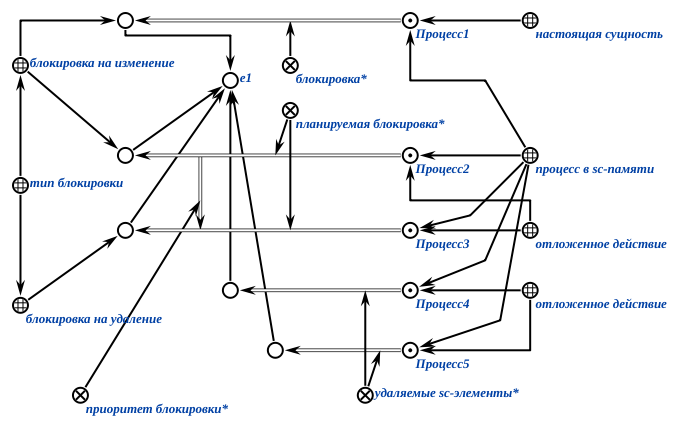
\includegraphics[width=0.7\textwidth]{figures/plan_lock_1.png}
    \end{center}
    Из примера видно, что блокировки это достаточно сложная штука.
\end{frame}

\end{document}